\begin{frame}
\frametitle{Tête simplifiée / Description}
\begin{columns}
\column{0.55\textwidth}
\scalebox{0.8}{\begin{minipage}{1.25\textwidth}
\begin{itemize}
\item Tête humaine simplifiée contenant un cerveau ;
\item $19\,413$ tétraèdres découpés ;
\item Permittivités relatives :
\begin{itemize}
\item Cerveau : 52 ;
\item Crâne : 11 ;
\end{itemize}
\item Condition limite absorbante (PML de Bérenger) ;
\item Antenne dipôle planaire rayonnant à 1 GHz (PEC) ;
\item Source : carré de côté 1 mm ;
\item Facteur d'échelle d'ordre 100 : favorise le GD ;
\item Forme d'onde (10 ns) : Gaussienne modulée
\end{itemize}
\end{minipage}}
\vfill
\begin{figure}
	\centering
		\begin{tikzpicture}[scale=0.5]
		\begin{axis}[
		axis lines=middle,
		xlabel=$ct$, x label style={at={(axis cs:3.3,0)},anchor=north},
		ylabel=$0$, y label style={at={(axis cs:0,-0.1)},anchor=east},
		xmin=-0.3,xmax=3.3,ymin=-1.1,ymax=1.1,
		xtick={0,1,...,4},%ytick={0,0.5,1},
		x post scale=1.5,
		y post scale=1,
		%legend style={at={(axis cs:0.9,0.2)},anchor=south west}
		]

		\addplot+[
		mark=none,
		color=gray,
		dotted, thick,
		samples=200,
		domain=0:3
		]
		{exp(-((x-1.448)/0.5509)^2)};

		\addplot+[
		thick,
		mark=none,
		color=red,
		samples=500,
		domain=0:3
		] table {../gauss_mod.plt};
		%{exp(-((x-1.448)/0.5509)^2)*sin(2*3.14159*10/3*(x-1.448))};

		%\node[anchor=east] (a) at (axis cs:0.9893456647,0.5){};
		%\node[anchor=west] (b) at (axis cs:1.9066543353,0.5){};
		%\draw[arrows={latex-latex}](a)--node[midway,below]{$2 \sqrt{\ln 2} \tau$}(b);

		\node[anchor=east] (c) at (axis cs:0,1){};
		\node[anchor=west] (d) at (axis cs:1.448,1){};
		\draw[dotted](c)--(d);

		%\node[anchor=east] (e) at (axis cs:0,0.5){};
		%\node[anchor=west] (f) at (axis cs:0.9893456647,0.5){};
		%\draw[dotted](e)--(f);

		\node[anchor=north] (g) at (axis cs:1.448,0){};
		\node[anchor=south] (h) at (axis cs:1.448,1){};
		\draw[dotted](g)--(h);

		%\node[anchor=north west] at (axis cs:1.448,0){$t_A$};
		%\node[anchor=north west] at (axis cs:0,1){$A$};

		\end{axis}
		\end{tikzpicture}
\end{figure}
\column{0.45\textwidth}
\begin{figure}
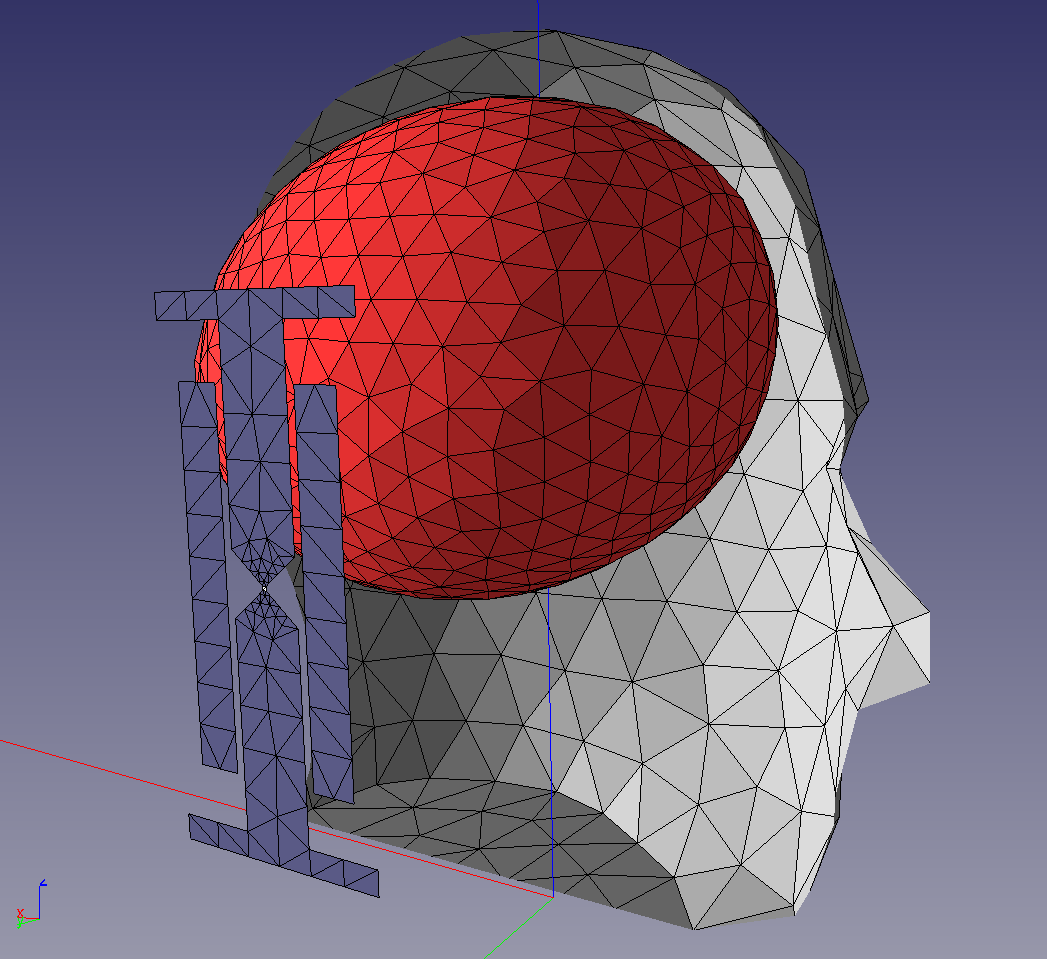
\includegraphics[width=0.9\textwidth]{../img/scene_brain}
\end{figure}
\vskip-1em
\begin{figure}
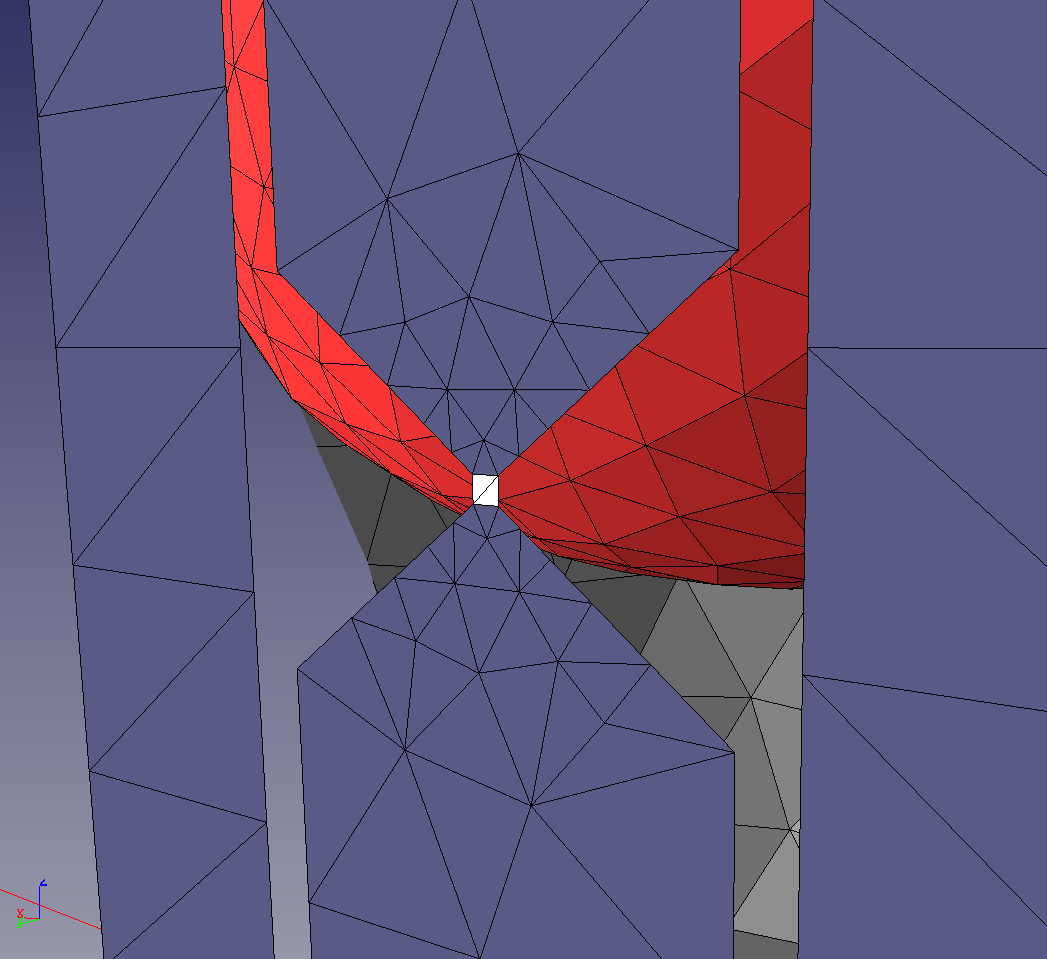
\includegraphics[width=0.9\textwidth,trim={0 200 0 200},clip]{../img/scene_brain_zoom}
\end{figure}
\end{columns}
\vfill
\end{frame}

